\documentclass[fleqn]{beamer}\usepackage[]{graphicx}\usepackage[]{color}
% maxwidth is the original width if it is less than linewidth
% otherwise use linewidth (to make sure the graphics do not exceed the margin)
\makeatletter
\def\maxwidth{ %
  \ifdim\Gin@nat@width>\linewidth
    \linewidth
  \else
    \Gin@nat@width
  \fi
}
\makeatother

\definecolor{fgcolor}{rgb}{0.345, 0.345, 0.345}
\newcommand{\hlnum}[1]{\textcolor[rgb]{0.686,0.059,0.569}{#1}}%
\newcommand{\hlstr}[1]{\textcolor[rgb]{0.192,0.494,0.8}{#1}}%
\newcommand{\hlcom}[1]{\textcolor[rgb]{0.678,0.584,0.686}{\textit{#1}}}%
\newcommand{\hlopt}[1]{\textcolor[rgb]{0,0,0}{#1}}%
\newcommand{\hlstd}[1]{\textcolor[rgb]{0.345,0.345,0.345}{#1}}%
\newcommand{\hlkwa}[1]{\textcolor[rgb]{0.161,0.373,0.58}{\textbf{#1}}}%
\newcommand{\hlkwb}[1]{\textcolor[rgb]{0.69,0.353,0.396}{#1}}%
\newcommand{\hlkwc}[1]{\textcolor[rgb]{0.333,0.667,0.333}{#1}}%
\newcommand{\hlkwd}[1]{\textcolor[rgb]{0.737,0.353,0.396}{\textbf{#1}}}%
\let\hlipl\hlkwb

\usepackage{framed}
\makeatletter
\newenvironment{kframe}{%
 \def\at@end@of@kframe{}%
 \ifinner\ifhmode%
  \def\at@end@of@kframe{\end{minipage}}%
  \begin{minipage}{\columnwidth}%
 \fi\fi%
 \def\FrameCommand##1{\hskip\@totalleftmargin \hskip-\fboxsep
 \colorbox{shadecolor}{##1}\hskip-\fboxsep
     % There is no \\@totalrightmargin, so:
     \hskip-\linewidth \hskip-\@totalleftmargin \hskip\columnwidth}%
 \MakeFramed {\advance\hsize-\width
   \@totalleftmargin\z@ \linewidth\hsize
   \@setminipage}}%
 {\par\unskip\endMakeFramed%
 \at@end@of@kframe}
\makeatother

\definecolor{shadecolor}{rgb}{.97, .97, .97}
\definecolor{messagecolor}{rgb}{0, 0, 0}
\definecolor{warningcolor}{rgb}{1, 0, 1}
\definecolor{errorcolor}{rgb}{1, 0, 0}
\newenvironment{knitrout}{}{} % an empty environment to be redefined in TeX

\usepackage{alltt}

% \usefonttheme[onlylarge]{structuresmallcapsserif}
\usefonttheme[onlysmall]{structurebold}
\usepackage[normalem]{ulem} % use normalem to protect \emph
\newcommand\hl{\bgroup\markoverwith
  {\textcolor{yellow}{\rule[-.5ex]{2pt}{2.5ex}}}\ULon}
\usepackage{amsmath,amssymb}
\usepackage{booktabs}
\usepackage{graphicx}
\usepackage{longtable}
\usepackage{lscape}
\usepackage[authoryear]{natbib}
\usepackage{mdframed}
\usepackage{array}
\usepackage{listings}
\usepackage{wasysym}
\usepackage{url}
\usepackage{multirow}
\usepackage{color}
\usepackage{qtree}
\usepackage{inconsolata}
\usepackage{framed}
\definecolor{shadecolor}{rgb}{1,0.8,0.3}
\usepackage[justification=centering]{caption}
\captionsetup{compatibility=false}
\usepackage{subcaption}
\usepackage{xcolor}
\usepackage{hyperref}
\hypersetup{colorlinks=true,linkcolor=blue}
\usepackage[space]{grffile}
\usefonttheme[onlymath]{serif}
% \usepackage{tikz}
% \usetikzlibrary{calc,matrix}
\usepackage{sgame}
\usepackage{tikz}
\usetikzlibrary{trees}

\mode<presentation>
%\usetheme{Frankfurt}
\usetheme{boxes}
\usecolortheme{beaver}
%\usetheme{Singapore}
%\usetheme{Hannover}

\newcommand*{\captionsource}[2]{%
  \caption[{#1}]{%
    #1%
    \\\hspace{\linewidth}%
    {\small\textbf{Source:} #2}%
  }%
}

\newenvironment{changemargin}[2]{%
  \begin{list}{}{%
    \setlength{\topsep}{0pt}%
    \setlength{\leftmargin}{#1}%
    \setlength{\rightmargin}{#2}%
    \setlength{\listparindent}{\parindent}%
    \setlength{\itemindent}{\parindent}%
    \setlength{\parsep}{\parskip}%
  }%
  \item[]}{\end{list}}

%Then \begin{changemargin}{-1cm}{-1cm} makes the margin 1 cm wider on either side of the page until \end{changemargin} appears.

\beamertemplatenavigationsymbolsempty
\setbeamertemplate{blocks}[rounded]
\newenvironment<>{block_code}[1]{%
  \setbeamercolor{block title}{fg=white,bg=black}%
  \begin{block}#2{#1}}{\end{block}}

%--------------------------
% Reduce the spacing between R code and output
%--------------------------
\usepackage{etoolbox}
\makeatletter
\preto{\@verbatim}{\topsep=0pt \partopsep=0pt }
\makeatother

\renewenvironment{knitrout}{\setlength{\topsep}{0mm}}{}

%===================================
% Coloring change
%===================================
\definecolor{darkred}{rgb}{0.8,0,0}
\setbeamercolor{block title}{fg=darkred,bg=structure.fg!20!bg!50!bg}
\setbeamercolor{block body}{use=block title,bg=block title.bg}

\title{Monte Carlo Simulation}
\author{Taro Mieno}
\date{AECN 896-003: Applied Econometrics}
\everymath{\displaystyle}
\IfFileExists{upquote.sty}{\usepackage{upquote}}{}
\begin{document}
\begin{frame}
\titlepage
\end{frame}




\begin{frame}[c,fragile]
  \frametitle{Monte Carlo Simulation}

  \begin{block}{What is it?}
   \textcolor{blue}{test econometric theories (prediction)} via simulation
  \end{block}
  
\end{frame}

\begin{frame}[c,fragile]
  \frametitle{Monte Carlo Simulation}
  \begin{block}{How is it used in econometrics?}
    \begin{itemize}
      \item confirm ecoometric theory numerically
        \begin{enumerate}
          \item OLS estimators are unbiased if $E[u|x]=0$ along with other conditions (theory)
          \item I know the above theory is right, but let's check if it is true numerically
        \end{enumerate}
      \item You kind of sense that something in your data may cause problems, but there is no proven econometric theory about what's gonna happen (I used MC simulation for this purpose a lot)
      \item assist students in understanding econometric theories by providing actual numbers instead of a series of Greek letters
    \end{itemize}
  \end{block}
\end{frame}

\begin{frame}[c]
  \frametitle{Monte Carlo Simulation}
  \begin{block}{Question}
    Suppose you are interested in checking what happens to OLS estimators if $E[u|x]=0$ (the error term and $x$ are not correlated) is violated. \\\vspace{0.6cm}

    \textcolor{blue}{Can you use the real data to do this?}
  \end{block}
\end{frame}

\begin{frame}[c]
  \frametitle{Monte Carlo Simulation}
  \begin{block}{Key part of MC simulation}
    \textcolor{blue}{You} generate data (you have control over how data are generated)\\\vspace{0.6cm}

    \begin{itemize}
      \item You know the true parameter unlike the real data generating process
      \item You can change only the part that you want to change about data generating process and econometric methods with everything else fixed
    \end{itemize}
  \end{block}
\end{frame}

\begin{frame}[c]
  \frametitle{Generating data}
  \begin{block}{Pseudo random number generator}
     algorithm for generating a sequence of numbers whose properties \textcolor{blue}{approximate} the properties of sequences of random numbers
  \end{block}
\end{frame}

\begin{frame}[c,fragile]
  \frametitle{Examples in R: Uniform Distribution}
\begin{knitrout}\footnotesize
\definecolor{shadecolor}{rgb}{0.969, 0.969, 0.969}\color{fgcolor}\begin{kframe}
\begin{alltt}
  \hlkwd{runif}\hlstd{(}\hlnum{5}\hlstd{)} \hlcom{# default is min=0 and max=1}
\end{alltt}
\begin{verbatim}
[1] 0.11011017 0.19312151 0.20463320 0.05153304 0.75362836
\end{verbatim}
\end{kframe}
\end{knitrout}
\end{frame}

\begin{frame}[c,fragile]
  \frametitle{Examples in R: Uniform Distribution}
\begin{knitrout}\footnotesize
\definecolor{shadecolor}{rgb}{0.969, 0.969, 0.969}\color{fgcolor}\begin{kframe}
\begin{alltt}
  \hlstd{x} \hlkwb{<-} \hlkwd{runif}\hlstd{(}\hlnum{10000}\hlstd{)}
  \hlkwd{hist}\hlstd{(x)}
\end{alltt}
\end{kframe}

{\centering \includegraphics[width=2.5in,height=2.5in]{figure/unif2-1} 

}



\end{knitrout}
\end{frame}

%===================================
% Pseudo random number generator
%===================================
\begin{frame}[c,fragile]
  \frametitle{Pseudo random number generator}
  \begin{itemize}
    \item Pseudo random number generators are not really random number generators
    \item What numbers you will get are pre-determined
    \item What numbers you will get can be determined by setting a \textcolor{blue}{seed}
    \item An example:
\begin{knitrout}\footnotesize
\definecolor{shadecolor}{rgb}{0.969, 0.969, 0.969}\color{fgcolor}\begin{kframe}
\begin{alltt}
    \hlkwd{set.seed}\hlstd{(}\hlnum{2387438}\hlstd{)}
    \hlkwd{runif}\hlstd{(}\hlnum{5}\hlstd{)}
\end{alltt}
\begin{verbatim}
[1] 0.0474233 0.7116970 0.4066674 0.2422949 0.3567480
\end{verbatim}
\end{kframe}
\end{knitrout}
    \item What benefits does setting a seed have?
  \end{itemize}
\end{frame}

\begin{frame}[c,fragile]
  \frametitle{Examples in R: Normal Distribution}
\begin{knitrout}\footnotesize
\definecolor{shadecolor}{rgb}{0.969, 0.969, 0.969}\color{fgcolor}\begin{kframe}
\begin{alltt}
    \hlstd{x} \hlkwb{<-} \hlkwd{rnorm}\hlstd{(}\hlnum{10000}\hlstd{)} \hlcom{# default is mean=0,sd=1}

    \hlkwd{hist}\hlstd{(x)}
\end{alltt}
\end{kframe}

{\centering \includegraphics[width=2.5in,height=2.5in]{figure/normal-1} 

}



\end{knitrout}
\end{frame}

\begin{frame}[c,fragile]
  \frametitle{Examples in R: Normal Distribution}
\begin{knitrout}\footnotesize
\definecolor{shadecolor}{rgb}{0.969, 0.969, 0.969}\color{fgcolor}\begin{kframe}
\begin{alltt}
  \hlstd{x} \hlkwb{<-} \hlkwd{rnorm}\hlstd{(}\hlnum{10000}\hlstd{,}\hlkwc{mean}\hlstd{=}\hlnum{2}\hlstd{,}\hlkwc{sd}\hlstd{=}\hlnum{2}\hlstd{)} \hlcom{# mean=2,sd=2}
  \hlkwd{hist}\hlstd{(x)}
\end{alltt}
\end{kframe}

{\centering \includegraphics[width=2.5in,height=2.5in]{figure/normal2-1} 

}



\end{knitrout}
\end{frame}

\begin{frame}[c,fragile]
  \frametitle{Other distributions}
  \begin{itemize}
    \item Beta
    \item Chi-square
    \item F
    \item Logistic
    \item Log-normal
    \item many others
  \end{itemize}
\end{frame}

\begin{frame}[c,fragile]
  \frametitle{r,p,r,d}
  For each distribution, you have four different kinds of functions:
  \begin{itemize}
    \item $\textcolor{red}{p}norm$: distribution function
    \item $\textcolor{red}{q}norm$: quantile function
    \item $\textcolor{red}{d}norm$: density function
    \item $\textcolor{red}{r}norm$: random draw
  \end{itemize}
\end{frame}

%--------------------------
% pnorm examples
%--------------------------
\begin{frame}[c,fragile]
  \frametitle{$pnorm$}
  \only<1-1>{
\begin{knitrout}\footnotesize
\definecolor{shadecolor}{rgb}{0.969, 0.969, 0.969}\color{fgcolor}

{\centering 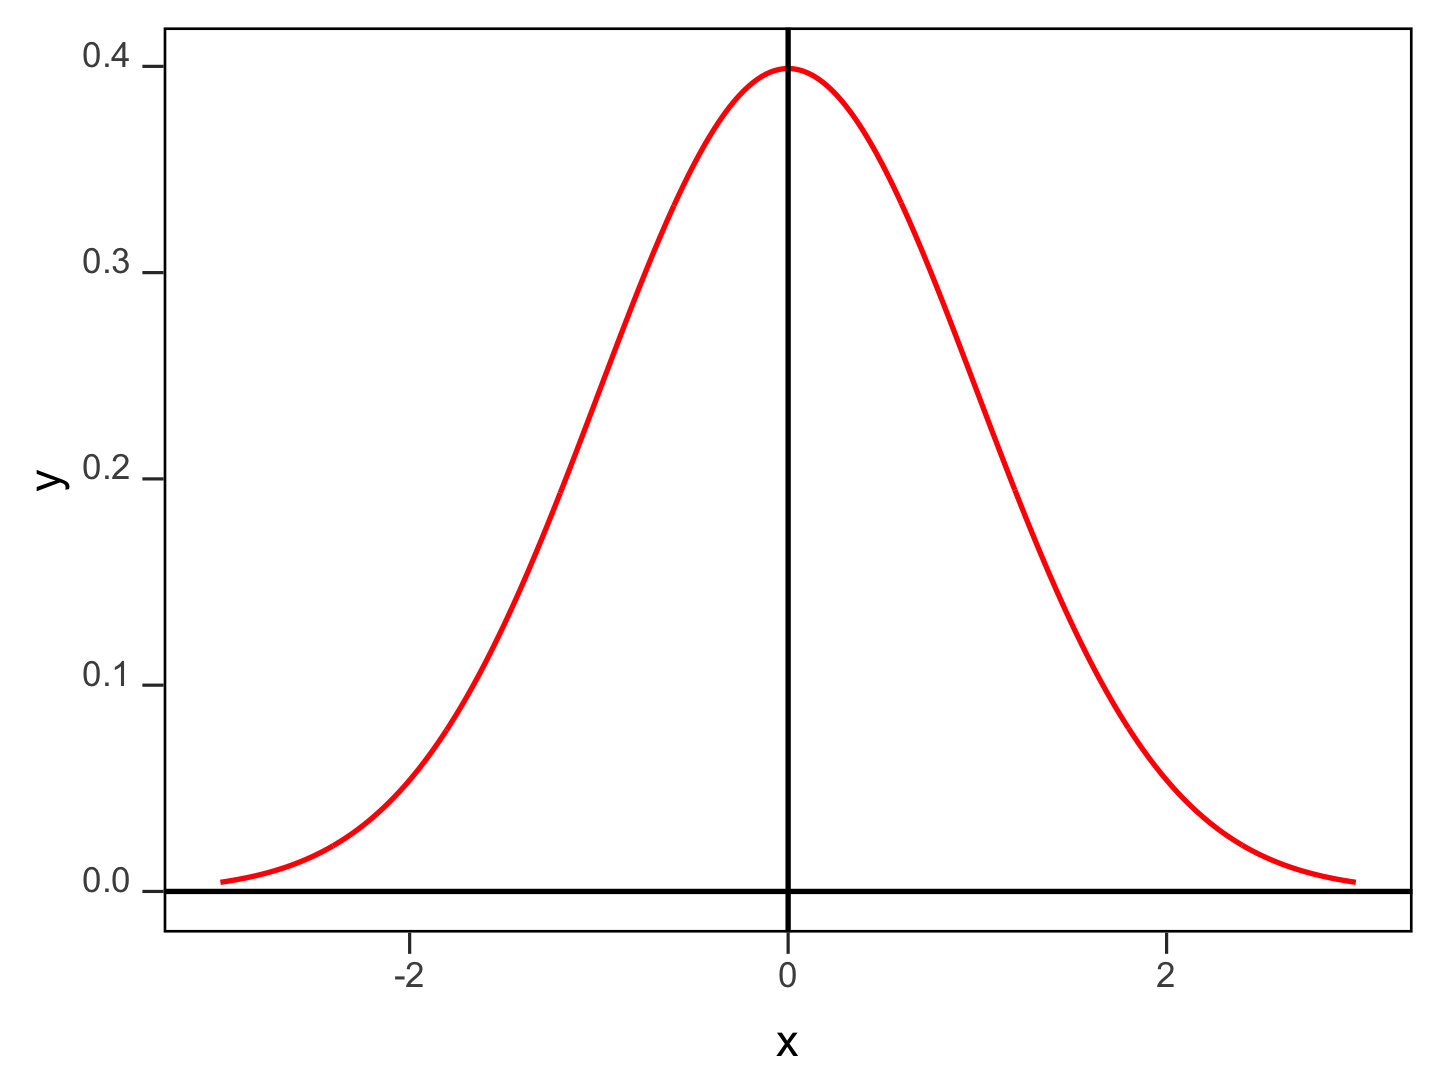
\includegraphics[width=3in,height=3in]{figure/pnorm-1} 

}



\end{knitrout}
  }
  \only<2->{
\begin{knitrout}\footnotesize
\definecolor{shadecolor}{rgb}{0.969, 0.969, 0.969}\color{fgcolor}

{\centering \includegraphics[width=3in,height=3in]{figure/pnorm_ex-1} 

}



\end{knitrout}
  }
\end{frame}

\begin{frame}[c,fragile]
  \frametitle{$qnorm$}
  \only<1-1>{
\begin{knitrout}\footnotesize
\definecolor{shadecolor}{rgb}{0.969, 0.969, 0.969}\color{fgcolor}

{\centering \includegraphics[width=3in,height=3in]{figure/qnorm-1} 

}



\end{knitrout}
  }
  \only<2-2>{
\begin{knitrout}\footnotesize
\definecolor{shadecolor}{rgb}{0.969, 0.969, 0.969}\color{fgcolor}

{\centering \includegraphics[width=3in,height=3in]{figure/qnorm_ex-1} 

}



\end{knitrout}
  }
  \only<3-3>{
\begin{knitrout}\footnotesize
\definecolor{shadecolor}{rgb}{0.969, 0.969, 0.969}\color{fgcolor}

{\centering \includegraphics[width=3in,height=3in]{figure/qnorm_ex_2-1} 

}



\end{knitrout}
  }

\end{frame}

% \begin{frame}[c,fragile]
%   \frametitle{$dnorm$}
%   << dnorm, echo=FALSE,out.height='3in',out.width='3in'>>=
%   x <- seq(-3,3,length=1000)
%   # x_ex <- 1
%   # y_ex <- dnorm(1)
%   pdf <- dnorm(x)
%   plot_data <- data.table(y=pdf,x=x)
%   ggplot()+
%     geom_line(data=plot_data,aes(y=y,x=x),color='red') +
%     # geom_line(data=data.table(y=seq(0,y_ex,length=1000),x=x_ex),
%     #   aes(y=y,x=x),linetype=2) +
%     # geom_line(data=data.table(x=seq(0,x_ex,length=1000),y=y_ex),
%     #   aes(y=y,x=x),linetype=2) +
%     geom_hline(yintercept=0) +
%     geom_vline(xintercept=0)

%   @
% \end{frame}

\begin{frame}[c]
  \frametitle{Monte Carlo Simulation: Steps}
  \begin{enumerate}
    \item specify the data generating process
    \item generate data based on the data generating process
    \item get an estimate based on the generated data (e.g. OLS, mean)
    \item repeat the above steps many many times
    \item compare your estimates with the true parameter
  \end{enumerate}
  \begin{block}{Question}
    Why do the steps $1-3$ many many times?
  \end{block}
\end{frame}

\begin{frame}[c]
  \frametitle{Monte Carlo Simulation: Example 1}
  \begin{block}{Question}
    Is sample mean really an unbiased estimator of the expected value? ($\frac{1}{n}\sum_{i=1}^n x_i = E[x]$ where $x_i$ is an independent random draw from the same distribution)
  \end{block}
\end{frame}

\begin{frame}[c,fragile]
  \frametitle{Sample Mean: Steps 1-3}
  \begin{block_code}{R code: Steps 1-3}

\begin{knitrout}\footnotesize
\definecolor{shadecolor}{rgb}{0.969, 0.969, 0.969}\color{fgcolor}\begin{kframe}
\begin{alltt}
  \hlcom{#--- steps 1 and 2:  ---#}
  \hlcom{# specify the data generating process and generate data}
  \hlstd{x} \hlkwb{<-} \hlkwd{runif}\hlstd{(}\hlnum{100}\hlstd{)} \hlcom{# Here, E[x]=0.5}

  \hlcom{#--- step 3 ---#}
  \hlcom{# calculate sample mean}
  \hlstd{mean_x} \hlkwb{<-} \hlkwd{mean}\hlstd{(x)}
  \hlstd{mean_x}
\end{alltt}
\begin{verbatim}
[1] 0.507078
\end{verbatim}
\end{kframe}
\end{knitrout}
  \end{block_code}
\end{frame}

% \newmdenv[linecolor=red,backgroundcolor=blue,frametitle=Infobox]{infobox}


\begin{frame}[c,fragile]
  \frametitle{Sample Mean: Step 4}
  \begin{itemize}
    \item Step 4: repeat the above steps many times (\textcolor{red}{why?})
    \item We use a \textcolor{blue}{loop} to do the same (similar) thing over and over again
  \end{itemize}

\begin{block_code}{R code: for loop}
  \footnotesize{
\begin{knitrout}\footnotesize
\definecolor{shadecolor}{rgb}{0.969, 0.969, 0.969}\color{fgcolor}\begin{kframe}
\begin{alltt}
  \hlcom{#--- the number of iterations ---#}
  \hlstd{B} \hlkwb{<-} \hlnum{1000}

  \hlcom{#--- repeat steps 1-3 B times ---#}
  \hlkwa{for} \hlstd{(i} \hlkwa{in} \hlnum{1}\hlopt{:}\hlstd{B)\{}
    \hlkwd{print}\hlstd{(i)} \hlcom{# print i}
  \hlstd{\}}
\end{alltt}
\end{kframe}
\end{knitrout}
  }
\end{block_code}

\end{frame}

\begin{frame}[c,fragile]
  \frametitle{Sample Mean: Step 4}
  \begin{block_code}{R code: Step 4}
   \footnotesize{
\begin{knitrout}\footnotesize
\definecolor{shadecolor}{rgb}{0.969, 0.969, 0.969}\color{fgcolor}\begin{kframe}
\begin{alltt}
  \hlcom{#--- the number of iterations ---#}
  \hlstd{B} \hlkwb{<-} \hlnum{1000}

  \hlcom{#--- create a storage that stores estimates ---#}
  \hlstd{estimate_storage_mean} \hlkwb{<-} \hlkwd{rep}\hlstd{(}\hlnum{0}\hlstd{,B)}

  \hlcom{#--- repeat steps 1-3 B times ---#}
  \hlkwa{for} \hlstd{(i} \hlkwa{in} \hlnum{1}\hlopt{:}\hlstd{B)\{}
    \hlcom{#--- steps 1 and 2:  ---#}
    \hlcom{# specify the data generating process and generate data}
    \hlstd{x} \hlkwb{<-} \hlkwd{runif}\hlstd{(}\hlnum{100}\hlstd{)} \hlcom{# Here, E[x]=0.5}

    \hlcom{#--- step 3 ---#}
    \hlcom{# calculate sample mean}
    \hlstd{mean_x} \hlkwb{<-} \hlkwd{mean}\hlstd{(x)}
    \hlstd{estimate_storage_mean[i]} \hlkwb{<-} \hlstd{mean_x}
  \hlstd{\}}
\end{alltt}
\end{kframe}
\end{knitrout}
  }
  \end{block_code}
\end{frame}

\begin{frame}[c,fragile]
  \frametitle{Sample Mean: Step 5}
  Compare your estimates with the true parameter
\begin{knitrout}\scriptsize
\definecolor{shadecolor}{rgb}{0.969, 0.969, 0.969}\color{fgcolor}\begin{kframe}
\begin{alltt}
  \hlkwd{mean}\hlstd{(estimate_storage_mean)}
\end{alltt}
\begin{verbatim}
[1] 0.500199
\end{verbatim}
\begin{alltt}
  \hlkwd{hist}\hlstd{(estimate_storage_mean)}
\end{alltt}
\end{kframe}

{\centering \includegraphics[width=2.3in,height=2.3in]{figure/step5-1} 

}



\end{knitrout}
\end{frame}

\begin{frame}[c]
  \frametitle{Monte Carlo Simulation: Example 2}
  \begin{block}{Question}
    What happens to $\beta_1$ if $E[u|x]\ne 0$ when estimating $y=\beta_0+\beta_1 x + u$?
  \end{block}
\end{frame}

\begin{frame}[c,fragile]
  \frametitle{Example 2}
  \begin{block_code}{R code: Example 2}
   \footnotesize{
\begin{knitrout}\footnotesize
\definecolor{shadecolor}{rgb}{0.969, 0.969, 0.969}\color{fgcolor}\begin{kframe}
\begin{alltt}
  \hlcom{#--- Preparation ---#}
  \hlstd{B} \hlkwb{<-} \hlnum{1000} \hlcom{# the number of iterations}
  \hlstd{N} \hlkwb{<-} \hlnum{100} \hlcom{# sample size}
  \hlstd{estimate_storage} \hlkwb{<-} \hlkwd{rep}\hlstd{(}\hlnum{0}\hlstd{,B)} \hlcom{# estimates storage}

  \hlcom{#--- repeat steps 1-3 B times ---#}
  \hlkwa{for} \hlstd{(i} \hlkwa{in} \hlnum{1}\hlopt{:}\hlstd{B)\{}
    \hlcom{#--- steps 1 and 2:  ---#}
    \hlstd{mu} \hlkwb{<-} \hlkwd{rnorm}\hlstd{(N)} \hlcom{# the common term shared by both x and u}
    \hlstd{x} \hlkwb{<-} \hlkwd{rnorm}\hlstd{(N)} \hlopt{+} \hlstd{mu} \hlcom{# independent variable}
    \hlstd{u} \hlkwb{<-} \hlkwd{rnorm}\hlstd{(N)} \hlopt{+} \hlstd{mu} \hlcom{# error}
    \hlstd{y} \hlkwb{<-} \hlnum{1} \hlopt{+} \hlstd{x} \hlopt{+} \hlstd{u} \hlcom{# dependent variable}
    \hlstd{data} \hlkwb{<-} \hlkwd{data.table}\hlstd{(}\hlkwc{y}\hlstd{=y,}\hlkwc{x}\hlstd{=x)}

    \hlcom{#--- OLS ---#}
    \hlstd{reg} \hlkwb{<-} \hlkwd{lm}\hlstd{(y}\hlopt{~}\hlstd{x,}\hlkwc{data}\hlstd{=data)} \hlcom{# OLS}
    \hlstd{estimate_storage[i]} \hlkwb{<-} \hlstd{reg}\hlopt{$}\hlstd{coef[}\hlstr{'x'}\hlstd{]}
  \hlstd{\}}
\end{alltt}
\end{kframe}
\end{knitrout}
  }
  \end{block_code}
\end{frame}

\begin{frame}[c,fragile]
  \frametitle{Example 2}
\begin{knitrout}\footnotesize
\definecolor{shadecolor}{rgb}{0.969, 0.969, 0.969}\color{fgcolor}\begin{kframe}
\begin{alltt}
  \hlkwd{hist}\hlstd{(estimate_storage)}
\end{alltt}
\end{kframe}

{\centering \includegraphics[width=2.5in,height=2.5in]{figure/ols_bias-1} 

}



\end{knitrout}
\end{frame}

\begin{frame}[c,fragile]
  \frametitle{MC Simulation: Exercise 1}
  \begin{block}{Problem}
    Using MC simulations, find out how the variance of error term affects the variance of OLS estimators
  \end{block}
  \begin{block}{Model set up}
  \vspace{-0.6cm}
    \begin{align*}
        y = \beta_0 + \beta_1 x + u_1 \\
        y = \beta_0 + \beta_1 x + u_2
    \end{align*}
  \vspace{-0.6cm}
  \begin{itemize}
    \item $x\sim N(0,1)$
    \item $u_1\sim N(0,1)$ and $u_2\sim N(0,9)$
    \item $E[u_1|x]=0$ and $E[u_2|x]=0$
  \end{itemize}
  \end{block}
  \begin{block}{Question}
    What should you expect?
  \end{block}
\end{frame}

%--- New Frame ---%

\begin{frame}
  \frametitle{Example 3: Estimation of the Variance of OLS Estimators}
  \begin{block}{True Variance of $\hat{\beta_1}$}
    \begin{align}
      V(\hat{\beta_1}) = \frac{\sigma^2}{\sum_{i=1}^n (x_i-\bar{x})^2} = \frac{\sigma^2}{SST_X}
    \end{align}
  \end{block}
  \begin{block}{Estimated Variance of $\hat{\beta_1}$}
    \begin{align}
      \hat{V}(\hat{\beta_1}) =\frac{\hat{\sigma}^2}{SST_X} = \frac{\sum_{i=1}^n \hat{u}_i^2}{n-2} \times \frac{1}{SST_X}
    \end{align}
  \end{block}
\end{frame}

%--- New Frame ---%

\begin{frame}[c,fragile]
  \begin{block_code}{R code: Example 3}
   \footnotesize{
\begin{knitrout}\footnotesize
\definecolor{shadecolor}{rgb}{0.969, 0.969, 0.969}\color{fgcolor}\begin{kframe}
\begin{alltt}
  \hlkwd{set.seed}\hlstd{(}\hlnum{903478}\hlstd{)}

  \hlcom{#--- Preparation ---#}
  \hlstd{B} \hlkwb{<-} \hlnum{10000} \hlcom{# the number of iterations}
  \hlstd{N} \hlkwb{<-} \hlnum{100} \hlcom{# sample size}
  \hlstd{beta_storage} \hlkwb{<-} \hlkwd{rep}\hlstd{(}\hlnum{0}\hlstd{,B)} \hlcom{# estimates storage for beta}
  \hlstd{V_beta_storage} \hlkwb{<-} \hlkwd{rep}\hlstd{(}\hlnum{0}\hlstd{,B)} \hlcom{# estimates storage for V(beta)}
  \hlstd{x} \hlkwb{<-} \hlkwd{rnorm}\hlstd{(N)} \hlcom{# x values are the same for every iteration}
  \hlstd{SST_X}  \hlkwb{<-} \hlkwd{sum}\hlstd{((x}\hlopt{-}\hlkwd{mean}\hlstd{(x))}\hlopt{^}\hlnum{2}\hlstd{)}

  \hlcom{#--- repeat steps 1-3 B times ---#}
  \hlkwa{for} \hlstd{(i} \hlkwa{in} \hlnum{1}\hlopt{:}\hlstd{B)\{}
    \hlcom{#--- steps 1 and 2:  ---#}
    \hlstd{u} \hlkwb{<-} \hlnum{2}\hlopt{*}\hlkwd{rnorm}\hlstd{(N)} \hlcom{# error}
    \hlstd{y} \hlkwb{<-} \hlnum{1} \hlopt{+} \hlstd{x} \hlopt{+} \hlstd{u} \hlcom{# dependent variable}
    \hlstd{data} \hlkwb{<-} \hlkwd{data.frame}\hlstd{(}\hlkwc{y}\hlstd{=y,}\hlkwc{x}\hlstd{=x)}

    \hlcom{#--- OLS ---#}
    \hlstd{reg} \hlkwb{<-} \hlkwd{lm}\hlstd{(y}\hlopt{~}\hlstd{x,}\hlkwc{data}\hlstd{=data)} \hlcom{# OLS}
    \hlstd{beta_storage[i]} \hlkwb{<-} \hlstd{reg}\hlopt{$}\hlstd{coef[}\hlstr{'x'}\hlstd{]}
    \hlstd{V_beta_storage[i]} \hlkwb{<-} \hlkwd{vcov}\hlstd{(reg)[}\hlstr{'x'}\hlstd{,}\hlstr{'x'}\hlstd{]}
  \hlstd{\}}
\end{alltt}
\end{kframe}
\end{knitrout}
  }
  \end{block_code}
\end{frame}

%--- New Frame ---%

\begin{frame}[c,fragile]
  \frametitle{Example 3}
  \begin{block}{True Variance}
    \begin{align}
      V(\hat{\beta}) = 4/112.07 = 0.0357
    \end{align}
  \end{block}
  \begin{block_code}{check}
   \footnotesize{
\begin{knitrout}\footnotesize
\definecolor{shadecolor}{rgb}{0.969, 0.969, 0.969}\color{fgcolor}\begin{kframe}
\begin{alltt}
    \hlkwd{var}\hlstd{(beta_storage)}
\end{alltt}
\begin{verbatim}
[1] 0.03562348
\end{verbatim}
\end{kframe}
\end{knitrout}
  }
  \end{block_code}
\end{frame}

%--- New Frame ---%

\begin{frame}[c,fragile]
  \frametitle{Your Estimates of Variance of $\hat{\beta_1}$?}

  \footnotesize{
\begin{knitrout}\footnotesize
\definecolor{shadecolor}{rgb}{0.969, 0.969, 0.969}\color{fgcolor}\begin{kframe}
\begin{alltt}
\hlcom{#=== mean ===#}
\hlkwd{mean}\hlstd{(V_beta_storage)}
\end{alltt}
\begin{verbatim}
[1] 0.03579118
\end{verbatim}
\end{kframe}
\end{knitrout}

\begin{knitrout}\footnotesize
\definecolor{shadecolor}{rgb}{0.969, 0.969, 0.969}\color{fgcolor}

{\centering \includegraphics[width=2.5in,height=2.5in]{figure/unnamed-chunk-1-1} 

}



\end{knitrout}
  }
\end{frame}

% \begin{frame}[c,fragile]
%   \frametitle{Exercise 1: Solution}
%   \begin{block_code}{R code: Solution}
%   << sol, size='scriptsize'>>=
%   #--- Preparation ---#
%   B <- 1000 # the number of iterations
%   N <- 100 # sample size
%   estimate_storage <- matrix(0,B,2) # estimates storage

%   for (i in 1:B){
%     #--- generate data ---#
%     x <- rnorm(N) # independent variable
%     u_1 <- rnorm(N,sd=1) # error 1
%     u_2 <- rnorm(N,sd=3) # error 2
%     y_1 <- 1 + x + u_1 # dependent variable 1
%     y_2 <- 1 + x + u_2 # dependent variable 2
%     data <- data.table(y_1=y_1,y_2=y_2,x=x)

%     #--- OLS ---#
%     reg_1 <- lm(y_1~x,data=data) # OLS
%     reg_2 <- lm(y_2~x,data=data) # OLS

%     #--- store coef estimates ---#
%     estimate_storage[i,1] <- reg_1$coef['x'] # equation 1
%     estimate_storage[i,2] <- reg_2$coef['x'] # equation 2
%   }
%   @
%   \end{block_code}
% \end{frame}

% \begin{frame}[c,fragile]
%   \frametitle{Exercise 1: Solution}
%   \begin{block_code}{R code: Compare}
%   << compare_sol, out.height='2.2in',out.width='2.2in',size='scriptsize'>>=
%   #--- assign new names ---#
%   beta_1s <- estimate_storage[,1]
%   beta_2s <- estimate_storage[,2]

%   #--- mean ---#
%   mean(beta_1s)
%   mean(beta_2s)

%   #--- sd ---#
%   sd(beta_1s)
%   sd(beta_2s)
%   @
%   \end{block_code}
% \end{frame}

% \begin{frame}[c,fragile]
%   \frametitle{Visualization}
%   << compare_viz, echo=F, out.height='3in',out.width='3in'>>=
%   plot_data_1 <- data.table(x=beta_1s,type='Equation 1')
%   plot_data_2 <- data.table(x=beta_2s,type='Equation 2')
%   plot_data <- rbind(plot_data_1,plot_data_2)
%   ggplot(data=plot_data) +
%     geom_density(aes(x=x,fill=type),alpha=0.5) +
%     scale_fill_discrete(name='')+
%     xlab('Coefficient Estimate') +
%     theme(
%       legend.position='bottom'
%       )
%   @
% \end{frame}

\begin{frame}[c,fragile]
  \frametitle{MC Simulation: Exercise 2}
  \begin{block}{Problem}
    Using MC simulations, find out how the variation in $x$ affects the OLS estimators
  \end{block}
  \begin{block}{Model set up}
  \vspace{-0.6cm}
    \begin{align*}
        y = \beta_0 + \beta_1 x_1 + u \\
        y = \beta_0 + \beta_1 x_2 + u
    \end{align*}
  \vspace{-0.6cm}
  \begin{itemize}
    \item $x_1\sim N(0,1)$ and $x_2\sim N(0,9)$
    \item $u\sim N(0,1)$
    \item $E[u_1|x]=0$ and $E[u_2|x]=0$
  \end{itemize}
  \end{block}
  \begin{block}{Question}
    What should you expect?
  \end{block}
\end{frame}

% \begin{frame}[c,fragile]
%   \frametitle{Exercise 2: Solution}
%   \begin{block_code}{R code: Solution}
%   << sol_2, size='scriptsize'>>=
%   #--- Preparation ---#
%   B <- 1000 # the number of iterations
%   N <- 100 # sample size
%   estimate_storage <- matrix(0,B,2) # estimates storage

%   for (i in 1:B){
%     #--- generate data ---#
%     x_1 <- rnorm(N,sd=1) # indep var 1
%     x_2 <- rnorm(N,sd=3) # indep var 2
%     u <- rnorm(N) # error
%     y_1 <- 1 + x_1 + u # dependent variable 1
%     y_2 <- 1 + x_2 + u # dependent variable 2
%     data <- data.table(y_1=y_1,y_2=y_2,x_1=x_1,x_2=x_2)

%     #--- OLS ---#
%     reg_1 <- lm(y_1~x_1,data=data) # OLS
%     reg_2 <- lm(y_2~x_2,data=data) # OLS

%     #--- store coef estimates ---#
%     estimate_storage[i,1] <- reg_1$coef['x_1'] # equation 1
%     estimate_storage[i,2] <- reg_2$coef['x_2'] # equation 2
%   }
%   @
%   \end{block_code}
% \end{frame}

% \begin{frame}[c,fragile]
%   \frametitle{Exercise 2: Solution}
%   \begin{block_code}{R code: Compare}
%   << compare_sol_2, out.height='2.2in',out.width='2.2in',size='scriptsize'>>=
%   #--- assign new names ---#
%   beta_1s <- estimate_storage[,1]
%   beta_2s <- estimate_storage[,2]

%   #--- mean ---#
%   mean(beta_1s)
%   mean(beta_2s)

%   #--- sd ---#
%   sd(beta_1s)
%   sd(beta_2s)
%   @
%   \end{block_code}
% \end{frame}

% \begin{frame}[c,fragile]
%   \frametitle{Visualization}
%   << compare_viz_2, echo=F, out.height='3in',out.width='3in'>>=
%   plot_data_1 <- data.table(x=beta_1s,type='Equation 1')
%   plot_data_2 <- data.table(x=beta_2s,type='Equation 2')
%   plot_data <- rbind(plot_data_1,plot_data_2)
%   ggplot(data=plot_data) +
%     geom_density(aes(x=x,fill=type),alpha=0.5) +
%     scale_fill_discrete(name='')+
%     xlab('Coefficient Estimate') +
%     theme(
%       legend.position='bottom'
%       )
%   @
% \end{frame}


\end{document}

